\documentclass[12pt]{article}
\usepackage{design_ASC}
\hypersetup{
    colorlinks=true,
    linkcolor=cyan,
    filecolor=magenta,
    urlcolor=blue,}

% Subfigures
\usepackage{subfig}

\setlength\parindent{0pt} %% Do not touch this

%% -----------------------------
%% TITLE
%% -----------------------------
\title{Exercise List \#5} %% Assignment Title

\author{Victor F. Ferrari - RA 187890\\ %% Student name
vferrari@mpc.com.br\\
MO814A/MC937A - Topics in Computer Graphics\\ %% Code and course name
\textsc{Universidade Estadual de Campinas}
}

\date{\today} %% Change "\today" by another date manually
%% -----------------------------
%% -----------------------------

%% %%%%%%%%%%%%%%%%%%%%%%%%%
\begin{document}
\setlength{\droptitle}{-5em}    
%% %%%%%%%%%%%%%%%%%%%%%%%%%
\maketitle

% --------------------------
% Start here
% --------------------------

%%%%%%%%%%%%%%%
\section{Projection}
%%%%%%%%%%%%%%%

\subsection*{Question 1}
{\bfseries What are and when the anomalies of the perspective projection occur? Illustrate the cases.}

Anomalies of perspective projections are features of that type of projection that alter the objects from the original scene. These anomalies are defining characteristics of perspective projections, and are usually \textbf{not} a problem.

The first anomaly is called \textbf{foreshortening}, in which objects that are farther from the projection center appear smaller, which is coherent with the way human vision works. The projection is not only altering the location, but also the size of the object. This anomaly is represented in figure \ref{fig:anom1} in red.

Perspective projections use \textbf{vanishing points}, so parallel lines meet in a point at infinity. For each set of parallel lines there's a corresponding vanishing point, and up to 3 principal points (for each axis). This anomaly is represented in figure \ref{fig:anom1} in green (the second parallel line is the building rooftop line).

Another anomaly of this type of projection is called \textbf{view confusion}, and happens when objects behind the center of projection are projected upside down and backward.

The last anomaly is called \textbf{topological distortion} and is similar to the last one, but instead of an object being behind the viewer there's a line crossing a plane where the center of projection is, so going from the front of the viewer to the back of it. This is projected to an infinite line.

\begin{figure}
    \centering
    \subfloat[Foreshortening and Vanishing Points]{
    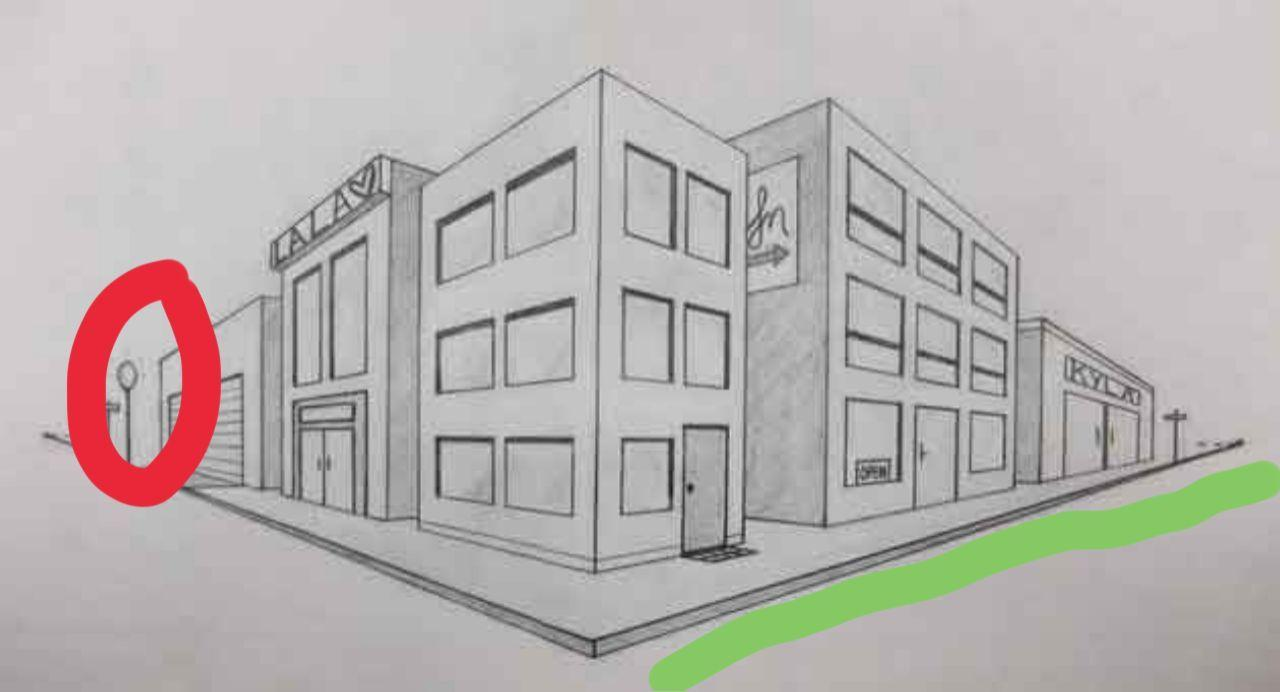
\includegraphics[width=0.5\textwidth]{images/persp.jpg}
    \label{fig:anom1}
    }
    \label{fig:anomalies}
    \caption{Anomalies}
\end{figure}

\subsection*{Question 2}
{\bfseries Compare perspective projections with parallel projections, their characteristics, advantages, and disadvantages.}

Parallel projections project the scene to an arbitrary plane without much distortion. Parallel lines in the scene are still parallel in the projection, and proportions are preserved. This is useful for technical projections that are highly depending of proportion and other applications where view realism is less important than representing accurately an object, but bad for applications that strive to portray a realistic view.

Perspective projections simulate human vision, so the resulting scene is similar to "looking through a window". A center of projection is used for this transformation. This type of projection causes many anomalies in relation to the original scene, as seen in the last question, then prioritizing realism over accuracy. In this projection, the proportions are not necessarily kept, and the size of the objects change (because of the foreshortening anomaly). This type of projection is useful for portraits, first-person games, animations and many other applications that require a more realistic portrayal of a scene, but bad if proportions and fidelity to the original scene are necessary, such as technical images, diagrams and such.

There's not one type of projection that is the best for every situation. Each application has a preferred projection type, as discussed.

\subsection*{Question 3}
{\bfseries What is the visualization pipeline in a graphics system? What are its steps?}

In a graphics system, the scene starts with its vertices in the object coordinate system (OCS). The objective is to transform these vertices to world coordinates, then to view coordinates and finally to \textbf{window} coordinates.

The first step is the transformation from OCS to WCS (world coordinates), and this last system can be very different from the first one. Afterwards, the next step is to transform the scene to \textbf{view coordinates}, which normally consists of projective transformations. The last coordinate conversion is from view coordinates to \textbf{DCS}, the window coordinates. This step consists of polygon or line clipping. Before clipping, the scene can also be mapped to an unit cube to facilitate clipping, and those are called \textbf{clip coordinates}.

Finally, with the scene in window coordinates, the last step is the \textbf{rasterization}, transforming the scene to an image with pixels, ending the transformation from vertices to pixels. In OpenGL, before clipping the \textit{vertex shader} does its processing, and after the rasterization the \textit{fragment shader} processes the image pixels.

\newpage

% %%%%%%%%%%%%%%%%%%%%%%%%%%%%%%%
\section{Lighting}
% %%%%%%%%%%%%%%%%%%%%%%%%%%%%%%%

\subsection*{Question 1}
{\bfseries What are Diffuse Reflection and Specular Reflection?}

Diffuse Reflection is a type of reflection such that an incident ray is reflected in all directions, so the light is \textbf{scattered}. So it is assumed that the surface also reflects all directions. In this case, the amount of reflected light is proportional to the incidence angle. This type of reflection is present in \textbf{rough surfaces}.

Specular Reflection, contrary to its diffuse counterpart, is a mirror-like reflection of light, adding highlights in the reflection direction. This is a "perfect" reflection, present in shiny objects. The intensity of the reflection depends on the intensity of the light source, the position of all related objects (the viewer, the source and the surface) and the surface (if it is smooth or shiny).

\begin{figure}
    \centering
    \subfloat[Diffuse Reflection]{
    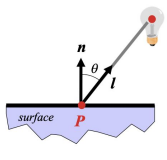
\includegraphics[width=0.4\textwidth]{images/diffuse.png}
    }
    \subfloat[Specular Reflection]{
    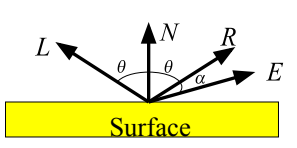
\includegraphics[width=0.5\textwidth]{images/specular.png}
    }
    \caption{Diffuse and specular reflections.}
    \label{fig:diff_spec}
\end{figure}

\subsection*{Question 2}
{\bfseries Which surfaces are called ideal diffuse reflectors? And ideal specular reflectors?}

Ideal diffuse reflectors are very rough surfaces that follow Lambert's law, so the ideal diffuse reflection is also called Lambertian reflection, where the light is scattered \textbf{uniformly} to all directions in a half-sphere over the surface. Materials such as chalk or marble are examples that are closer to an ideal lambertian reflector.

Ideal specular reflectors are surfaces that produce perfect reflections that follow the three laws of reflection, such as a mirror. In these cases, the reflection is completely directional, and the surfaces reproduce to the viewer what is in the exact same angle on the other side of the surface normal.

\subsection*{Question 3}
{\bfseries In Phong’s lighting equation, what is the component that allows you to manipulate specular reflection?}

Phong's lighting equation is as follows:
\[ I=k_aA+C(k_d(L\cdot N)+k_s(R\cdot E)^n) \]

This equation consists of three components for ambient, diffuse and specular lighting. The key to understanding each component is to check each variable and constant.

The specular component is:
\[ I_s=Ck_s(R\cdot E)^n \]

where $k_s$ is the specular reflection coefficient, $R$ is the reflected vector, $E$ is the vector representing the direction of the eye (viewer), $n$ is the specular exponent and $C$ is the light source intensity.

Since specular reflection is based in directional reflections and the position of both the viewer and the source (represented by the reflected vector) in relation to the object, this term can be identified as the one responsible for specular reflection. The product between the vectors are used to replace $\cos{\alpha}$, where $\alpha$ is the angle between the two.

\subsection*{Question 4}
{\bfseries The lighting model equation for a single light source is given by:

\[(k_aI_a + k_dI_l(N \cdot L)) + k_sI_l(N \cdot H)^{n_s}\]

Explain the meaning of each of the following parameters. Give the range of variation for each one
and explain what the effect of their change is on the final appearance of an object: $k_a$, $k_d$, $k_s$, $I_a$, $I_l$, and $n_s$.}

As briefly discussed in the answer to question 3, $n_s$ is the specular exponent and $k_s$ is the specular reflection coefficient. Similarly, $k_a$ and $k_d$ are the ambient and diffuse reflection coefficients, respectively. $I_a$ and $I_l$ are the intensity of ambient light and of the point light source, respectively.

The $k$ coefficients are properties of the surface, depending on intrinsic characteristic such as material. Their range is always between 0 and 1, so $0 \leq k_i \leq 1$ $\forall i \in \{a,d,s\}$. Changing the value of each component will increase or decrease the weight of that type of reflection in the lighting model: the higher the coefficient, more present is the corresponding reflection. An important property is the composition of both $k_d$ and $k_s$: they never exceed 1. So, $0 \leq k_d+k_a \leq 1$.

$I_a$ and $I_l$ represent intensity of light, so they are actually a vector of 3 values, corresponding to each color band in RGB. Those values are also normalized between 0 and 1. This term is multiplicative, so the intensity of the reflected light is proportional to these values. A higher ambient light intensity means higher reflected ambient light intensity, and therefore more ambient light. Similarly, higher light source intensity means stronger diffuse and specular reflections, the intensity of the resulting light for \textbf{both} reflections are stronger.

Finally, $n_s$ is also called "shininess coefficient", and its range is between 1 and $\infty$. The ideal specular reflector has $n_s=\infty$. The term $(N\cdot H)^{n_s}$ produces a curve for each value of $n_s$. The higher the exponent, the narrower the curve and the resulting specular highlight area is smaller. This can be good to make the object appear "shinier", especially in small values, but also can make the object darker, especially in larger values. This coefficient has no physical meaning, being fully empirical and mathematical.

\subsection*{Question 5}
{\bfseries How are the coefficients $k_a$, $k_d$ and $k_s$ and the parameter $n_s$ obtained?}

As discussed in the previous question, the $k$ coefficients are intrinsic of the object, but they (as with the $n_s$ parameter) do \textbf{not} have a physical meaning, being purely mathematical for the model to work and be configurable. Therefore, these coefficients are dependant on the situation, and are usually obtained \textbf{empirically}, either by testing or by checking previous results.

However, we still consider these coefficients as \textbf{object properties}, even if they aren't directly linked to physical aspects.

\subsection*{Question 6}
{\bfseries How are vectors $N$, $L$, and $H$ computed?}

The $N$ vector is the normalized normal vector to the surface at the current analyzed point. As such, it is a vector perpendicular to the surface at the current point. $L$ is the \textbf{incident ray} vector, so it is the vector from the current point to the light source, and can be computed in this way. It is also normalized.

Finally, $H$ is a term specific for the Blinn-Phong variation of the lighting equation, and is the "halfway" vector between the one representing the \textbf{viewer} ($V$) and $L$. As such, the vector is computed, if you already have $V$, by the following equation. As can be seen, this vector is also normalized.

\[H=\frac{L+V}{\lVert L+V \lVert}\]

\subsection*{Question 7}
{\bfseries What is the difference between calculating the specular component as in the above equation or using the vectors $R$ and $V$? How are these two vectors obtained?}

The main advantage of the Blinn-Phong variation is the \textbf{faster computation}. Using this variation, the computation of the $R$ vector is avoided, the only vectors needed are $N$, $L$ and $V$ directly, and the operation is straightforward. The former two are already used for the diffuse component, and the latter is easily obtained. 

Another difference lies in the specular exponent $n_s$. In this variation, the specular component has "more weight" than in the variation with $R$ and $V$. If $n$ is the exponent for the regular Phong equation, we have $n_s \simeq 4n$.

The $V$ vector is the normalized vector between the viewer and the current point, so it is the difference $V=C-P$, where $C$ is the camera position and $P$ is the current point. The computation of $R$ is a lot more expensive than the others, including $H$: $R$ is the difference between the component of $L$ that is perpendicular to the surface ($L_n$) and the component that is parallel to the surface ($L_p$). Note that $R$ requires a dot product, and $H$ doesn't.

\[R = L_n - L_p = 2(L\cdot N)N - L\]

It must be said that the Blinn-Phong equation is \textbf{not} equal to the original Phong equation, but is very similar, so they are usually used interchangeably.

\subsection*{Question 8}
{\bfseries In what situation can $L$ and $H$ (or $R$ and $V$) be considered as constant? What is the advantage of using these constant vectors? What is the disadvantage?}

Since $H$ depends only on $L$ and $V$, if those vectors are constant, $H$ is also constant. Those vectors can be considered as constant when they are very remote, such as at infinity or approaching infinity. In that case, both vectors converge in this remote distance, and so they can be considered constant for the entire frame. This can also happen when the light source and the viewer are in the same relative position.

In this case, $H$ can be computed once for the entire frame, and then used for every point. This is only possible for the Blinn-Phong variation, since in the original equation $R$ needs to be calculated for every point and depends on the surface curvature. In that case, $R$ is only constant when $L$ changes uniformly with the normal $N$.

The advantage to considering the vectors as constants is the efficiency gained by saving on computing a vector in each point of the frame. In higher resolutions, the gain is even more pronounced. The disadvantage is that this can cost visual quality or fidelity by making approximations. In practice, a light source and a viewer are never approaching infinity, so to make this quality cost null those points should be very far away.

\subsection*{Question 9}
{\bfseries What is the difference between a global lighting model and a local model? Explain.}

A global lighting model represents the interactions between every light source and the environment, so each point of the scene, trying to represent how the light would behave on a scene without individually modeling the interactions with objects. The object interaction results are a byproduct of this approach, and \textbf{light bounce} can be represented, with not only light effects from the light source but also reflected light from other objects. It is usually expensive and complex, but can produce realistic results. An example of global lighting models is \textbf{ray-tracing}.

A local lighting model tries to represent each interaction of light with an object, in contrast to the environment-focused approach of the global models. In this case, only the light that hits a surface and is transmitted to the eye is accounted for, so the result is a cheaper model, very used for real-time applications such as games. An example of local lighting models is the \textbf{Phong lighting model}.

\newpage

%%%%%%%%%%%%%%%%%%%%%%%%%%%%%%%%%%%
\section{Shading}
%%%%%%%%%%%%%%%%%%%%%%%%%%%%%%%%%%%

\subsection*{Question 1}
{\bfseries What are the advantages and disadvantages of Gouraud Shading over Flat (Faceted)? And Phong’s Shading over Gouraud?}

Gouraud Shading is a \textbf{per-vertex} shading method, where a color is assigned to each vertex and then interpolated to the rest of the polygon. In contrast, flat shading assumes one color per polygon. 

The advantages of Gouraud shading over Flat shading include the improved accuracy of the result by the improved \textbf{continuity} between polygons, since the transition doesn't have to be as harsh. This can be a huge improvement, depending on the application. The disadvantages lie on the new problems it introduces, such as \textbf{mach bands} and special cases in perspective projections, or in the fact that it is still a more expensive method than flat shading, and there are specific applications where the result is not better (if the normals at each vertex of a polygon are the same), so some time can possibly be lost. Still, if the issues can be resolved, it is still a better method than flat shading most of the time.

Phong's Shading is a \textbf{per-pixel} shading method, where a normal is assigned to each vertex and then interpolated to the rest of the polygon. The main difference from Gouraud Shading is that the normal is interpolated instead of the color itself, and so the lighting equations are solved for each pixel instead of each vertex.

The advantages of Phong shading over Gouraud include the much improved results (harder to diferentiate low-polygon and high-polygon models), and highlights are captured much better. Since the normals are interpolated, the specular lighting component can be included, while that may not be possible in Gouraud shading. The main disadvantage of this method is the computational cost, being a more expensive model especially on high-resolution scenes, because a lighting equation needs to be solved for every pixel. Also, discontinuities may arise because of shared vertices, and the interpolation depends on the orientation of the polygon.

\subsection*{Question 2}
{\bfseries Build a data structure to represent a grid of quadrilaterals. Write a program to calculate the shading of the mesh represented by your data structure. (Just in pseudo-code)}

To represent a quadrilateral, multiple approaches are possible. An approach is the one used by older versions of OpenGL, with a \textbf{Quad} primitive structure. This structure would have 4 coplanar 3D points ordered counter-clockwise with the sides of the quad, along with optionally 4 normal values (one for each vertex). Another approach is to use 2 triangles, as is the standard for modern OpenGL. For the remainder of this question, the first approach will be used.

A grid of quadrilaterals can be defined as a vector or list of quads. Adjacent quads can be modeled by duplicating the common vertices. Another approach is to have a container with each quad, including references to adjacent quad containers (one for each direction) to preserve topological information, and this can be done with or without vertex duplication (but then the quads would not have 4 points). For the pseudocode, vertex duplication is considered, with a vector, and this structure is called \textbf{QuadGrid}.

The pseudocode for shading this grid with \textbf{Gouraud Shading} is in the following block:
\begin{verbatim}
    g: QuadGrid with n Quads in a vector.
    for each quad q in g:
        for each v in q.vertices:
            S(v) = lighting equation solution for v (shade).
            
        min = min_y(q.vertices)
        max = max_y(q.vertices)
        Initialize edges for scan with both edges with min as endpoint.
        
        # Interpolate linearly the shades.
        # Scan line: min y to max y: go through edges.
        # AB and CD may not be the same edges in each line.
        for y = min.y to max.y:
            Change leftmost and/or rightmost edge if at the end of one.
        
            P = point of the leftmost edge (AB) with P.y = y.
            Q = point of the rightmost edge (CD) with Q.y = y
            
            # Lerping edges.
            # d: euclidean distance.
            t(AB) = d(A,P)/d(A,B)
            t(CD) = d(C,Q)/d(C,D)
            S(P) = t(AB)S(A) + (1-t(AB))S(B)
            S(Q) = t(CD)S(C) + (1-t(CD))S(D)
            
            # Lerping interior.
            for x = P.x to Q.x:
                Z = point (x,y)
                t(PQ) = (x - P.x)/(Q.x - P.x)
                S(Z) = t(PQ)S(P) + (1-t(PQ))S(Q)
\end{verbatim}

In the end, every pixel will have its shade. Changing the structure to the graph-like, the way of going through the quads would be different, and without vertex duplication an indexing method would need to be implemented.

\subsection*{Question 3}
{\bfseries Describe the main steps of Shading Flat, Gouraud and Phong.}

Flat shading is a \textbf{per-polygon} method. A single lighting equation is solved per polygon, in an arbitrary point (usually the center), and then this color is applied to the rest of the polygon. This process is repeated for each polygon.

Gouraud Shading is a \textbf{per-vertex} shading method, where a color is assigned to each vertex and then interpolated to the rest of the polygon. So, based on the normals and position of each vertex, a color is assigned, so there is one lighting equation solved per vertex of a polygon, and then this color is interpolated linearly to the rest of the polygon, first through the edges, then by scanlines to fill the polygon.

Phong's Shading is a \textbf{per-pixel} shading method, where a normal is assigned to each vertex and then interpolated to the rest of the polygon. So normals are assumed in each vertex, then they are interpolated to the rest of the polygon \textbf{before} solving any lighting equations and assigning colors. After the interpolation, one lighting equation is solved per pixel to assign its color.

\end{document}